\section{Appendix B}
\label{appendix:b}

This appendix includes supplimentary pictures for the report.

\begin{figure}[ht!]
    \begin{center}
    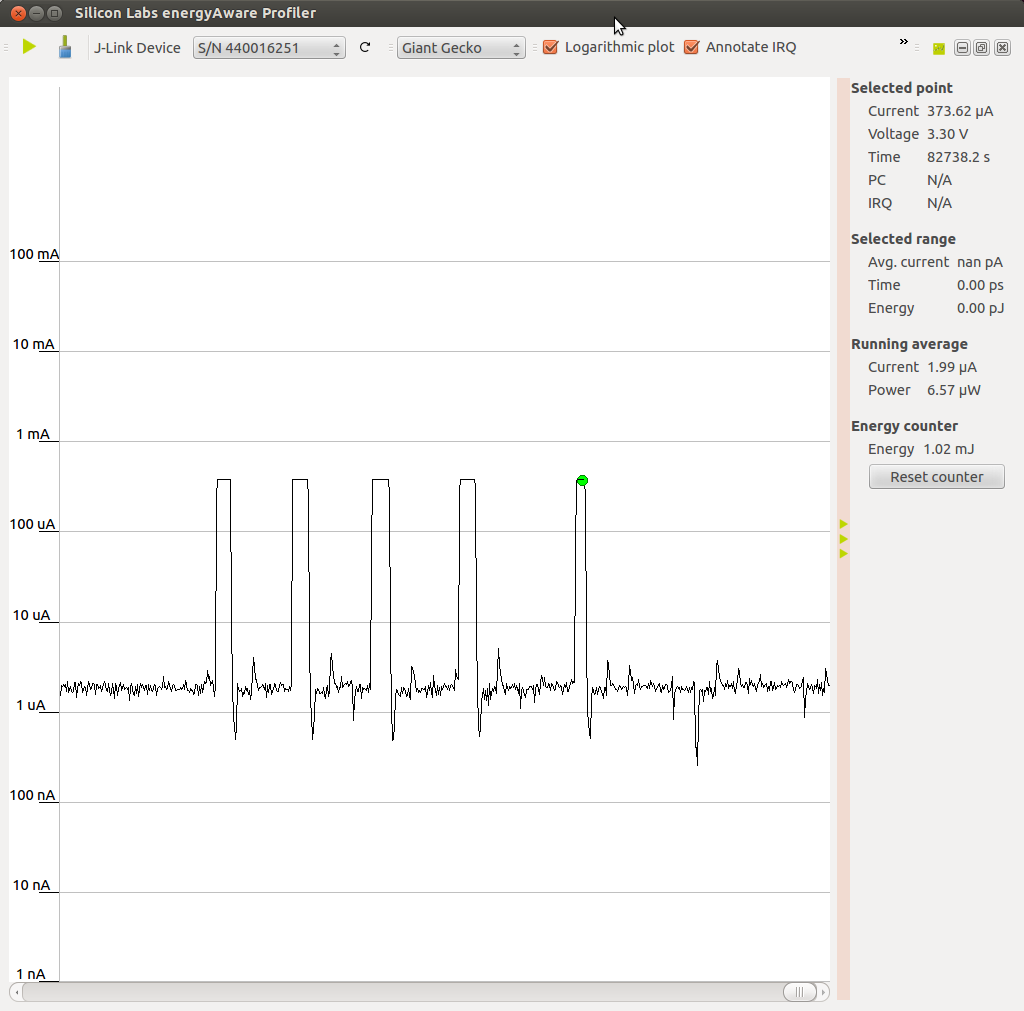
\includegraphics[width=0.8\textwidth]{assets/img/no_opening_seq.png}
    \caption{eAProfiler reading with no opening sequence. Each spike is a reset.}
    \label{fig:no_opening_seq}
    \end{center}
\end{figure}

\begin{figure}[ht!]
    \begin{center}
    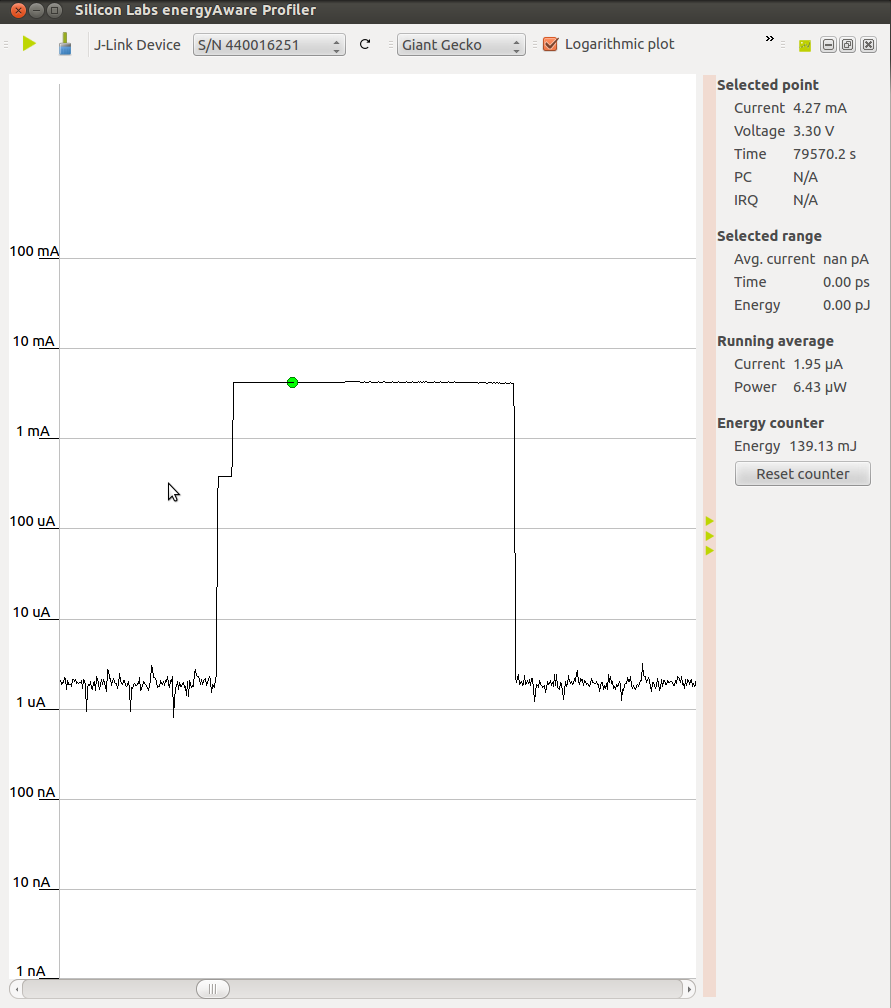
\includegraphics[width=0.8\textwidth]{assets/img/opening_seq.png}
    \caption{eAProfiler reading with opening sequence. The spike is a reset.}
    \label{fig:opening_seq}
    \end{center}
\end{figure}

\begin{figure}[ht!]
    \begin{center}
    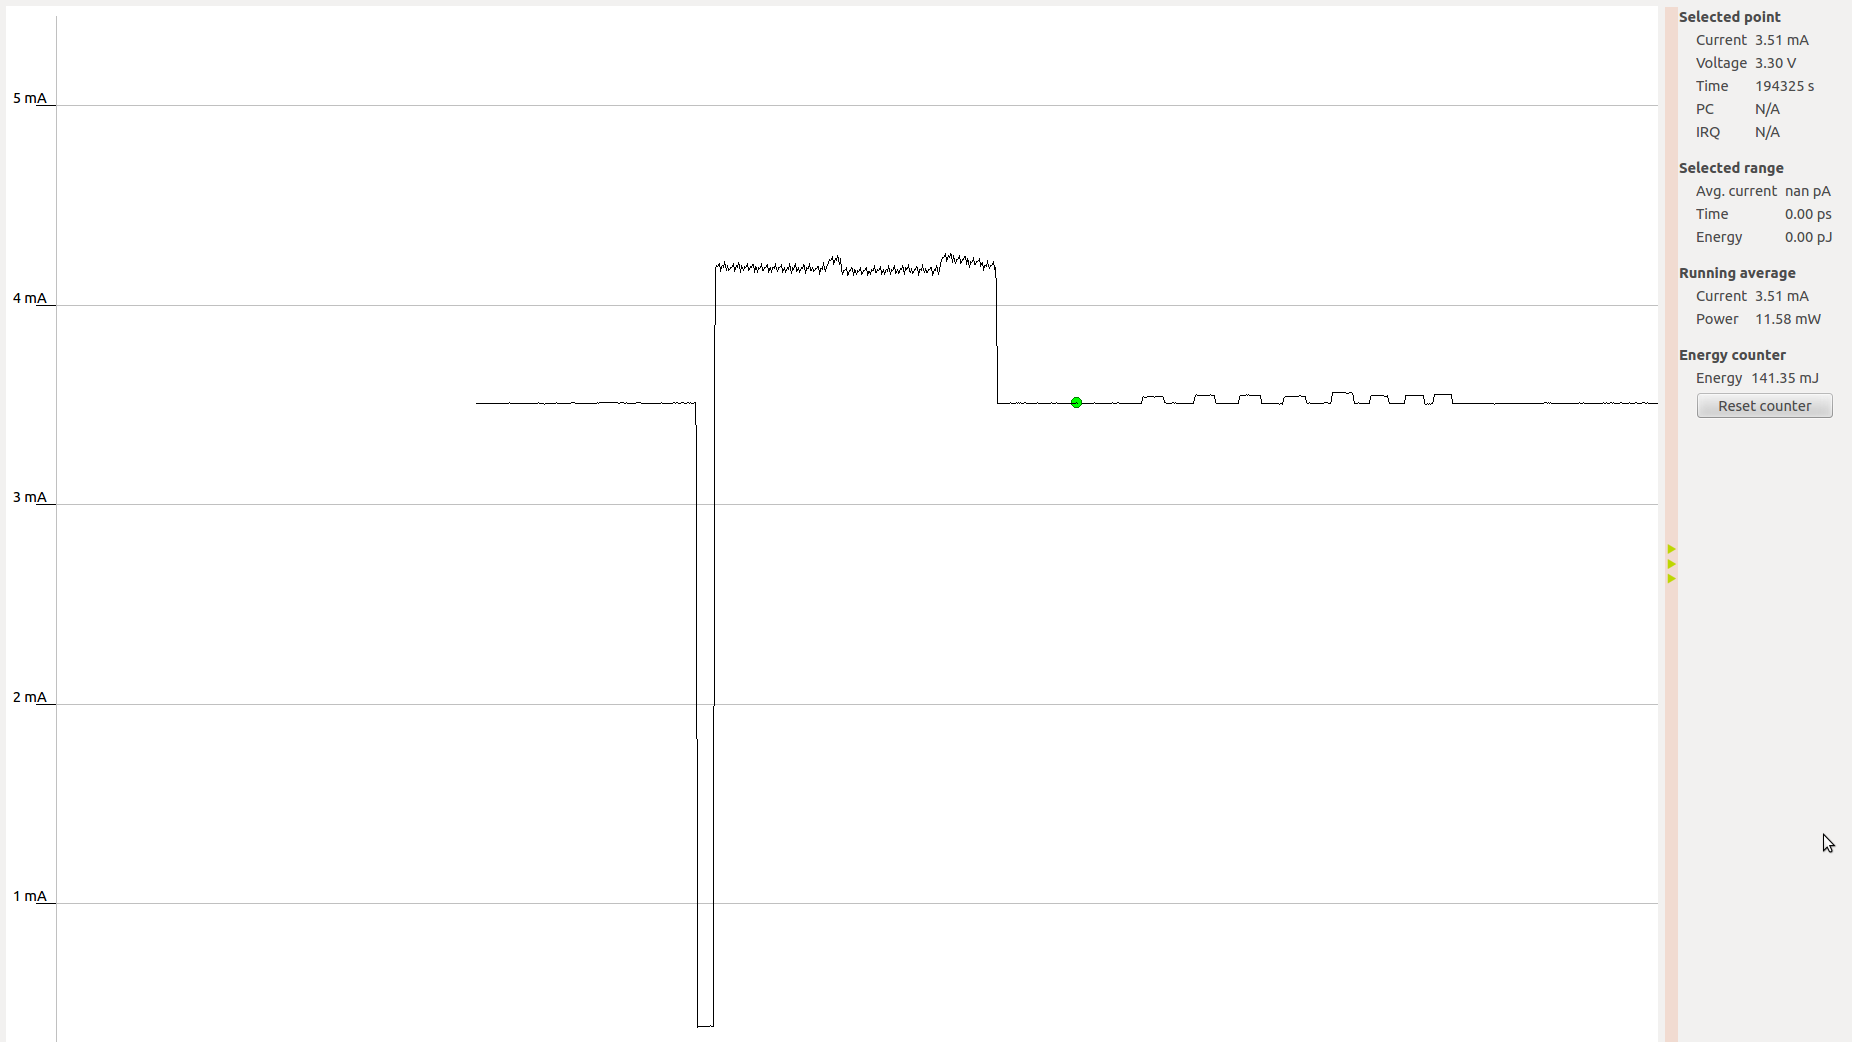
\includegraphics[width=0.8\textwidth]{assets/img/polling.png}
    \caption{Energy usage when using polling for I/O. The plateau is the oh so energy consuming boot sequence, and the small bumps are button pushes.}
    \label{fig:polling_io}
    \end{center}
\end{figure}

\begin{figure}[ht!]
    \begin{center}
    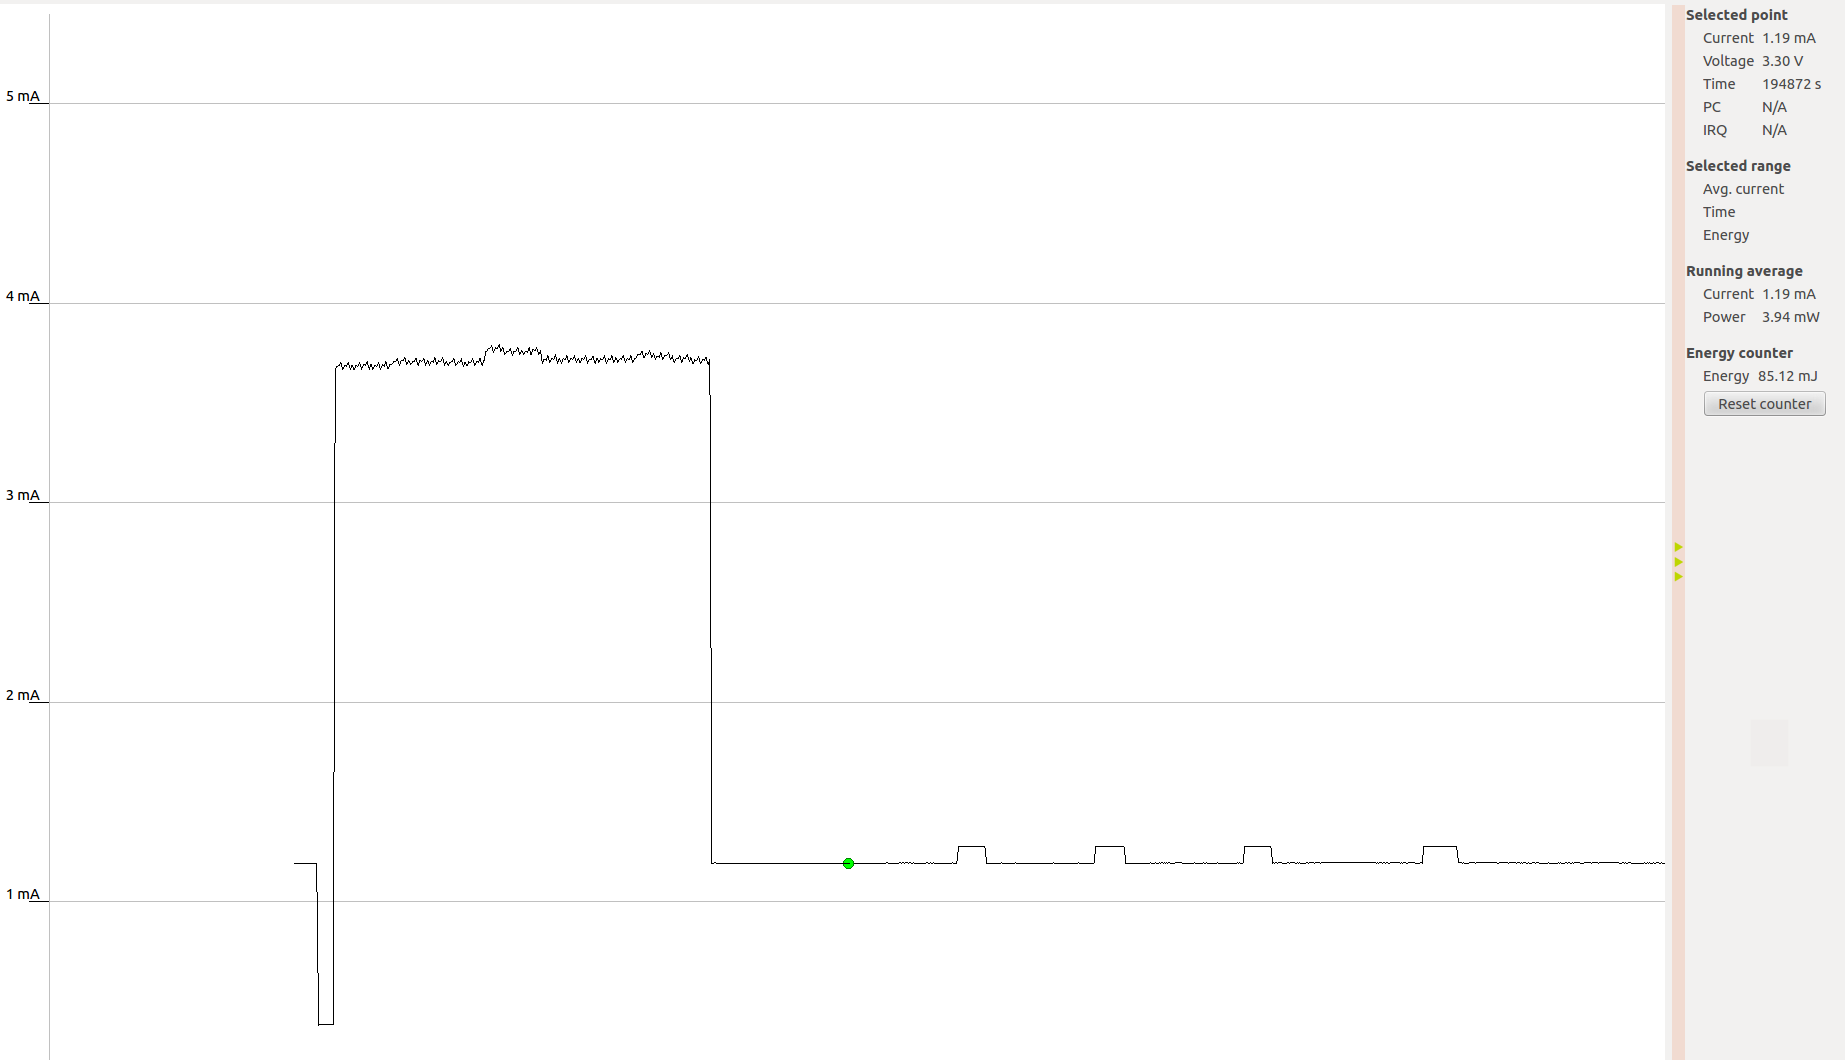
\includegraphics[width=0.8\textwidth]{assets/img/interrupt_regular_sleep.png}
    \caption{Energy usage when using interrupts to detect I/O events, and letting the CPU sleep in between}
    \label{fig:interrupt_io}
    \end{center}
\end{figure}

\begin{figure}[ht!]
    \begin{center}
    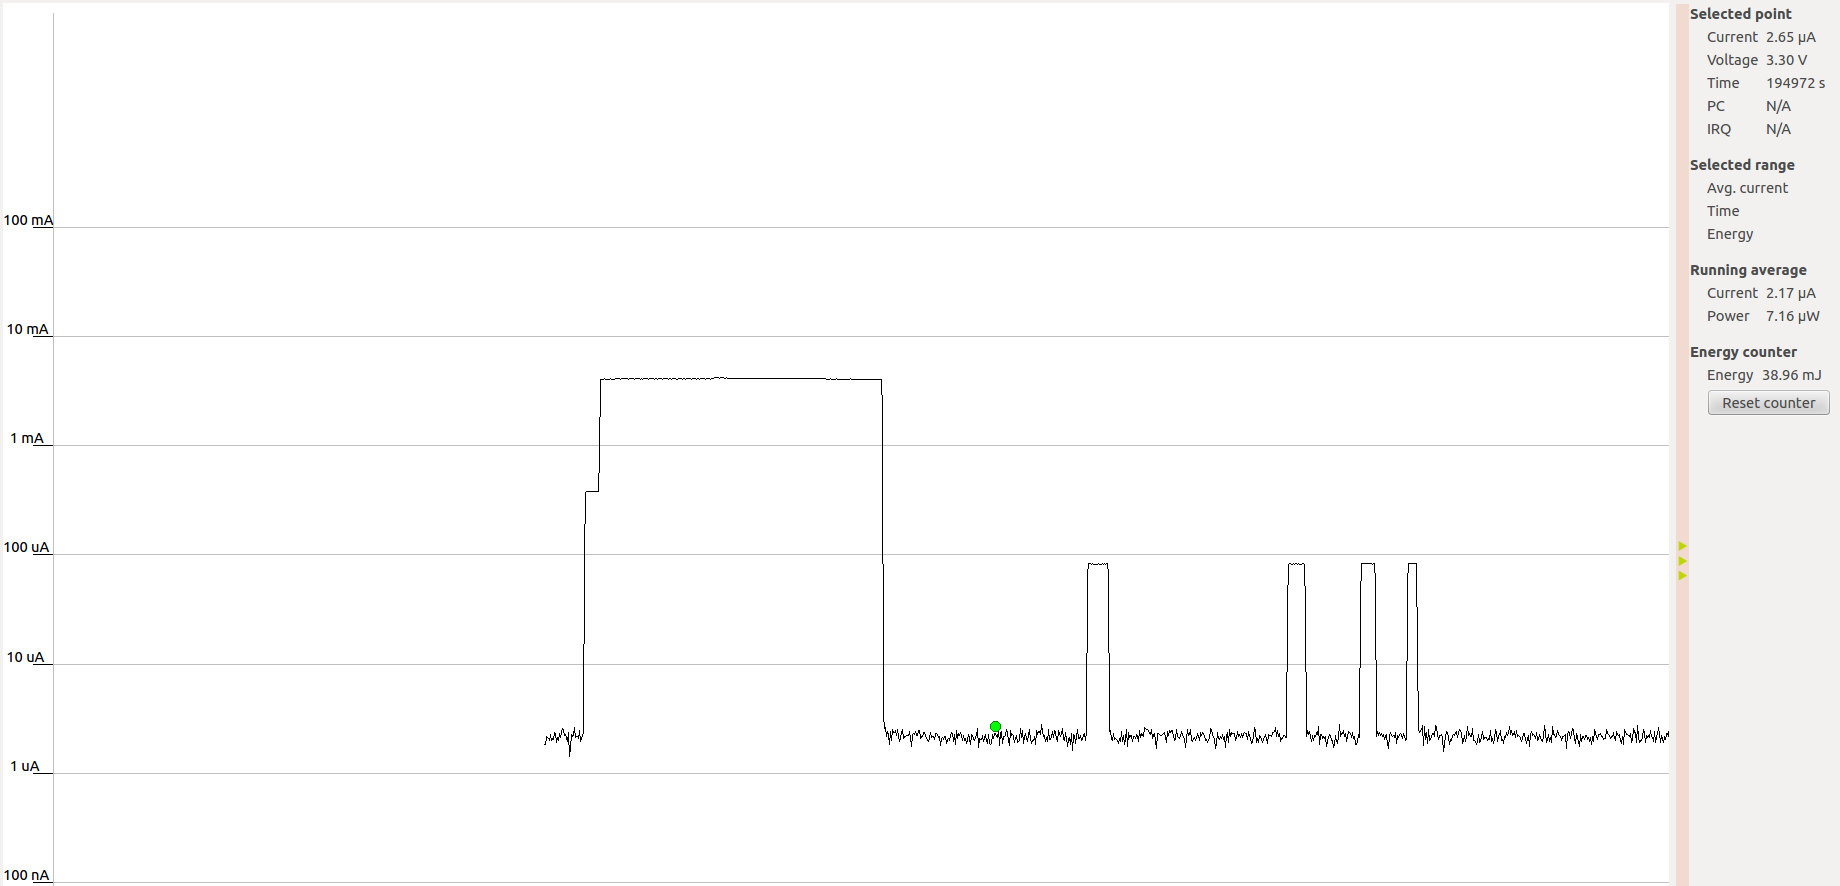
\includegraphics[width=0.8\textwidth]{assets/img/interrupt_deep_sleep.png}
    \caption{Energy usage when using interrupts to wake up the CPU for responding to I/O events. Sleep mode is set to Energy Mode 2}
    \label{fig:interrupt_io_deep_sleep}
    \end{center}
\end{figure}
